% Options for packages loaded elsewhere
\PassOptionsToPackage{unicode}{hyperref}
\PassOptionsToPackage{hyphens}{url}
%
\documentclass[
]{book}
\usepackage{amsmath,amssymb}
\usepackage{iftex}
\ifPDFTeX
  \usepackage[T1]{fontenc}
  \usepackage[utf8]{inputenc}
  \usepackage{textcomp} % provide euro and other symbols
\else % if luatex or xetex
  \usepackage{unicode-math} % this also loads fontspec
  \defaultfontfeatures{Scale=MatchLowercase}
  \defaultfontfeatures[\rmfamily]{Ligatures=TeX,Scale=1}
\fi
\usepackage{lmodern}
\ifPDFTeX\else
  % xetex/luatex font selection
\fi
% Use upquote if available, for straight quotes in verbatim environments
\IfFileExists{upquote.sty}{\usepackage{upquote}}{}
\IfFileExists{microtype.sty}{% use microtype if available
  \usepackage[]{microtype}
  \UseMicrotypeSet[protrusion]{basicmath} % disable protrusion for tt fonts
}{}
\makeatletter
\@ifundefined{KOMAClassName}{% if non-KOMA class
  \IfFileExists{parskip.sty}{%
    \usepackage{parskip}
  }{% else
    \setlength{\parindent}{0pt}
    \setlength{\parskip}{6pt plus 2pt minus 1pt}}
}{% if KOMA class
  \KOMAoptions{parskip=half}}
\makeatother
\usepackage{xcolor}
\usepackage{longtable,booktabs,array}
\usepackage{calc} % for calculating minipage widths
% Correct order of tables after \paragraph or \subparagraph
\usepackage{etoolbox}
\makeatletter
\patchcmd\longtable{\par}{\if@noskipsec\mbox{}\fi\par}{}{}
\makeatother
% Allow footnotes in longtable head/foot
\IfFileExists{footnotehyper.sty}{\usepackage{footnotehyper}}{\usepackage{footnote}}
\makesavenoteenv{longtable}
\usepackage{graphicx}
\makeatletter
\def\maxwidth{\ifdim\Gin@nat@width>\linewidth\linewidth\else\Gin@nat@width\fi}
\def\maxheight{\ifdim\Gin@nat@height>\textheight\textheight\else\Gin@nat@height\fi}
\makeatother
% Scale images if necessary, so that they will not overflow the page
% margins by default, and it is still possible to overwrite the defaults
% using explicit options in \includegraphics[width, height, ...]{}
\setkeys{Gin}{width=\maxwidth,height=\maxheight,keepaspectratio}
% Set default figure placement to htbp
\makeatletter
\def\fps@figure{htbp}
\makeatother
\setlength{\emergencystretch}{3em} % prevent overfull lines
\providecommand{\tightlist}{%
  \setlength{\itemsep}{0pt}\setlength{\parskip}{0pt}}
\setcounter{secnumdepth}{5}
\usepackage{booktabs}
\ifLuaTeX
  \usepackage{selnolig}  % disable illegal ligatures
\fi
\usepackage[]{natbib}
\bibliographystyle{plainnat}
\IfFileExists{bookmark.sty}{\usepackage{bookmark}}{\usepackage{hyperref}}
\IfFileExists{xurl.sty}{\usepackage{xurl}}{} % add URL line breaks if available
\urlstyle{same}
\hypersetup{
  pdftitle={``源计划''开放课题},
  pdfauthor={SHUD研究组},
  hidelinks,
  pdfcreator={LaTeX via pandoc}}

\title{``源计划''开放课题}
\author{SHUD研究组}
\date{2024-08-01}

\begin{document}
\maketitle

{
\setcounter{tocdepth}{1}
\tableofcontents
}
\hypertarget{ux7b80ux4ecb}{%
\chapter{简介}\label{ux7b80ux4ecb}}

``源计划''可视为我们研究组的开放课题项目,它的目标是以项目的形式为组内成员和合作者提供自主研究资金,以支持他们的科研梦想。我们希望这个计划能为年轻人提供一个''起点'',一个开始追逐梦想的地方,支持他们敢于梦想,并从这里走得更远。

\textbf{资助金额2-4万;执行期1-2年。申请者一般为大学三年级或以上,研究生2年级或以上学生}

\hypertarget{ux7ecfux8d39ux8bf4ux660e}{%
\section{经费说明}\label{ux7ecfux8d39ux8bf4ux660e}}

\begin{enumerate}
\def\labelenumi{\arabic{enumi}.}
\item
  ``源计划''的经费来自于项目组现有项目(母项目)经费和商业赞助。
\item
  \textbf{经费的支出方式必须严格遵守中国科学院西北生态环境资源研究院的经费管理规定,并借鉴母项目的经费预算情况。}
\item
  经费不可转移,并购买的固定资产设备会受到中国科学院西北生态环境资源研究院的经费管理制度的监管。
\item
  经费只能用于进行指定科学研究任务。
\item
  所有经费不拨款,支出需通过中国科学院西北生态环境资源研究院。
\item
  经费由接受资助的人员使用,但在管理程序上,需要PI的授权签字。
\end{enumerate}

\hypertarget{ux6210ux679cux5f52ux5c5e}{%
\section{成果归属}\label{ux6210ux679cux5f52ux5c5e}}

\begin{enumerate}
\def\labelenumi{\arabic{enumi}.}
\tightlist
\item
  \textbf{被资助的研究者在项目成果上有优先署名权}。受资助者主动撰写学术论文,则受资助者应当成为第一作者。受资助者放弃领衔撰写学术论文的机会,则该研究成果可由其他成员领衔撰写,受资助者可获得共同第一作者署名。
\item
  \textbf{成果产出由本研究组及中国科学院西北生态环境资源研究院共同拥有}。成果的第一或第二单位应当是``中国科学院西北生态环境资源研究院'',本组PI应当是成果的通讯作者或共同通讯作者。
\item
  \textbf{在成果中应当体现母项目和赞助的资助}。成果的第一资助来源信息应当是本研究组指定的项目。
\end{enumerate}

\hypertarget{ux9879ux76eeux798fux5229}{%
\section{项目福利}\label{ux9879ux76eeux798fux5229}}

\begin{enumerate}
\def\labelenumi{\arabic{enumi}.}
\tightlist
\item
  \textbf{自主支配的科研经费}:项目成员有权自主决定如何使用提供的经费。
\item
  \textbf{学术指导}:项目执行全程,受资助者都可以从本研究组获得学术指导。包括研究方法、中英文写作等。
\item
  \textbf{学术资源}:作为我们团队的研究生或科研助理,受资助者将享受我们团队和单位提供的\textbf{学术(文献和社交网络)、数据、计算(超算)、软件(商业、私有、AI)资源}等。本组的研究资源可参考:\url{https://www.shud.xyz/book_lab/servers}
\item
  \textbf{成果产出}:包括但不限于学术论文、专利、软件著作权、数据产权、著作权、其他知识产权收益等。
\item
  \textbf{实现你的梦想}:我们想资助的是你的科研梦想。
\end{enumerate}

\hypertarget{ux7533ux8bf7ux65b9ux5f0f}{%
\chapter{申请方式}\label{ux7533ux8bf7ux65b9ux5f0f}}

\hypertarget{ux6750ux6599}{%
\section{材料}\label{ux6750ux6599}}

\begin{enumerate}
\def\labelenumi{\arabic{enumi}.}
\tightlist
\item
  项目选题可直接申请已有的指南任务,或者自由选题。
\item
  自由选题仅限\textbf{大气、水文、地理、遥感、生态方向},以及与\textbf{以上方向有交叉}的计算机、高性能计算、人工智能、软硬件设备等。恕能力限制,其他方向无法提供学术指导和经费支持。
\item
  经费预算数额不超过4万元;项目的一般执行期为1年。请根据项目研究内容做合理经费预算和时间规划。
\item
  申请材料:

  \begin{itemize}
  \tightlist
  \item
    申请书:请参考国家自然科学基金申请书范本。其中包括了研究意义、研究现状、研究思路、研究内容、待解决的科学问题、研究详细技术路线、拟取得的科研成果、详细的项目时间表、经费预算、现有研究基础等。申请书应包含项目执行的时间表,详细规划任务完成的重要时间节点,时间规划应详细到季度。
  \item
    学术简历:

    \begin{itemize}
    \tightlist
    \item
      姓名、照片、联系方式
    \item
      教育经历
    \item
      工作经历,可包括全职、兼职、实习等。
    \item
      已有研究成果:可包括论文、专利、软著、软件源代码、博客、公众号文章等
    \item
      其他:其他表现个人能力和性格的内容。
    \end{itemize}
  \end{itemize}
\item
  项目经费的可支出额度比例不高于项目执行进度比例。
\end{enumerate}

\hypertarget{ux7533ux8bf7ux6d41ux7a0b}{%
\section{申请流程}\label{ux7533ux8bf7ux6d41ux7a0b}}

\begin{enumerate}
\def\labelenumi{\arabic{enumi}.}
\tightlist
\item
  申请方式:申请书+申请人个人简历,发送至PI邮箱:\href{mailto:shulele@lzb.ac.cn}{\nolinkurl{shulele@lzb.ac.cn}}
\item
  2024年度项目申请截止时间2024年8月15日。
\item
  2024年9月1日之前组织视频答辩。答辩后,本研究组对申请书给出回复意见,请根据回复意见对申请书进行修改。
\item
  视频答辩后30天给出明确是否资助的结果。
\item
  项目受资助之后,立即开始执行。
\end{enumerate}

\hypertarget{ux7533ux8bf7ux8868}{%
\section{申请表}\label{ux7533ux8bf7ux8868}}

最新申请表下载:\url{https://shud.xyz/openfund.docx}

个人简历模版(仅供参考):\url{https://shud.xyz/CV_template.docx}

\hypertarget{ux4efbux52a1ux8fdbux5ea6ux8bf4ux660e}{%
\chapter{任务进度说明}\label{ux4efbux52a1ux8fdbux5ea6ux8bf4ux660e}}

\hypertarget{ux6750ux6599-1}{%
\section{材料}\label{ux6750ux6599-1}}

\begin{enumerate}
\def\labelenumi{\arabic{enumi}.}
\tightlist
\item
  项目选题可直接申请已有的指南任务,或者自由选题。
\item
  自由选题仅限\textbf{大气、水文、地理、遥感、生态方向},以及与\textbf{以上方向有交叉}的计算机、高性能计算、人工智能、软硬件设备等。恕能力限制,其他方向无法提供学术指导和经费支持。
\item
  经费预算数额不超过4万元;项目的一般执行期为1年。请根据项目研究内容做合理经费预算和时间规划。
\item
  申请材料:

  \begin{itemize}
  \tightlist
  \item
    申请书:请参考国家自然科学基金申请书范本。其中包括了研究意义、研究现状、研究思路、研究内容、待解决的科学问题、研究详细技术路线、拟取得的科研成果、详细的项目时间表、经费预算、现有研究基础等。申请书应包含项目执行的时间表,详细规划任务完成的重要时间节点,时间规划应详细到季度。
  \item
    学术简历:

    \begin{itemize}
    \tightlist
    \item
      姓名、照片、联系方式
    \item
      教育经历
    \item
      工作经历,可包括全职、兼职、实习等。
    \item
      已有研究成果:可包括论文、专利、软著、软件源代码、博客、公众号文章等
    \item
      其他:其他表现个人能力和性格的内容。
    \end{itemize}
  \end{itemize}
\item
  项目经费的可支出额度比例不高于项目执行进度比例。
\end{enumerate}

\hypertarget{ux7533ux8bf7ux6d41ux7a0b-1}{%
\section{申请流程}\label{ux7533ux8bf7ux6d41ux7a0b-1}}

\begin{enumerate}
\def\labelenumi{\arabic{enumi}.}
\tightlist
\item
  申请方式:申请书+申请人个人简历,发送至PI邮箱:\href{mailto:shulele@lzb.ac.cn}{\nolinkurl{shulele@lzb.ac.cn}}
\item
  2024年度项目申请截止时间2024年8月15日。
\item
  2024年9月1日之前组织视频答辩。答辩后,本研究组对申请书给出回复意见,请根据回复意见对申请书进行修改。
\item
  视频答辩后30天给出明确是否资助的结果。
\item
  项目受资助之后,立即开始执行。
\end{enumerate}

\hypertarget{ux7533ux8bf7ux8868-1}{%
\section{申请表}\label{ux7533ux8bf7ux8868-1}}

最新申请表下载:\url{https://shud.xyz/openfund.docx}

个人简历可参考:\url{https://shud.xyz/CV_template.docx}

\hypertarget{ux9879ux76eeux9884ux7b97}{%
\chapter{项目预算}\label{ux9879ux76eeux9884ux7b97}}

\hypertarget{ux7ecfux8d39ux9884ux7b97ux8981ux6c42}{%
\section{经费预算要求}\label{ux7ecfux8d39ux9884ux7b97ux8981ux6c42}}

\begin{enumerate}
\def\labelenumi{\arabic{enumi}.}
\tightlist
\item
  劳务费,支出不超过每月1000元的劳务费,以\textbf{科研助理月津贴}的形式发放。
\item
  版面费、专利申请费、软著申请费等出版费用。
\item
  差旅费用。包括学术会议的注册费、食宿和路费。野外工作使用的野外装备、租车、加油、过路费、住宿费等。
\item
  办公和计算费用:一般办公使用的数据存储设备、一般电脑耗材;租用服务器、超算、网络磁盘等支出;
\item
  奖金:不超过5000元的奖金。奖金数额不体现在申请书中。
\end{enumerate}

\hypertarget{ux652fux51faux6761ux4ef6}{%
\section{支出条件}\label{ux652fux51faux6761ux4ef6}}

为防止经费滥用,研究经费需要在完成特定任务量后方可开始支取。请参考下表中``可支出条件''。

\begin{longtable}[]{@{}cccr@{}}
\toprule\noalign{}
类别 & 支出理由 & 可支出条件 & 预算上限(元) \\
\midrule\noalign{}
\endhead
\bottomrule\noalign{}
\endlastfoot
劳务费 & 个人劳务支出 & 项目完成60\%以上 & 12000 \\
出版费用 & 成果发表 & 文章接受,以正式发票为准 & 16000 \\
差旅费 & 学术交流 & 项目完成50\%以上 & 5000 \\
材料/计算 & 计算费、野外装备、文具等 & 项目完成20\%以上 & 2000 \\
奖金 & 优秀项目 & 项目100\%,档案备份 & 5000 \\
\textbf{总额} & & & \textbf{40000} \\
\end{longtable}

\hypertarget{ux9879ux76eeux7ed3ux9898}{%
\chapter{项目结题}\label{ux9879ux76eeux7ed3ux9898}}

\hypertarget{ux6b63ux5e38ux7ed3ux9898}{%
\section{正常结题}\label{ux6b63ux5e38ux7ed3ux9898}}

\begin{enumerate}
\def\labelenumi{\arabic{enumi}.}
\tightlist
\item
  一份正式结题报告。
\item
  成果正式发表、受理或接受。形式包括研究论文,软著,专利。
\item
  提交可重复、可核查的研究资料档案。包括但不限于:

  \begin{enumerate}
  \def\labelenumii{\arabic{enumii}.}
  \tightlist
  \item
    源代码:模型,软件,脚本等
  \item
    数据:原始数据,数据中间过程,
  \item
    图件、照片、视频等
  \item
    沟通邮件
  \end{enumerate}
\end{enumerate}

\hypertarget{ux7ecfux8d39ux7ed3ux4f59}{%
\section{经费结余}\label{ux7ecfux8d39ux7ed3ux4f59}}

\begin{enumerate}
\def\labelenumi{\arabic{enumi}.}
\tightlist
\item
  部分经费可以津贴或奖金形式发放,但其数额不超过预算但单项和总额限制。
\item
  无法支取的经费,将直接回收。
\end{enumerate}

\hypertarget{ux9879ux76eeux4e2dux6b62ux673aux5236}{%
\section{项目中止机制}\label{ux9879ux76eeux4e2dux6b62ux673aux5236}}

\begin{enumerate}
\def\labelenumi{\arabic{enumi}.}
\tightlist
\item
  项目执行期,受资助人发现难度超过其能力范围,可申请中止。
\item
  项目进度未能按照申请书进度完成,且无合理理由,项目将被中止,并需返回所有固定资产设备。
\item
  项目中止后,所有数据和已有工作必须完整上交。后续由其他研究者继续研究。如发表成果,将根据项目前期工作量和价值,判定是否在成果中体现原项目受资助人的贡献。
\end{enumerate}

\hypertarget{ux9009ux9898ux6307ux5357}{%
\chapter{选题指南}\label{ux9009ux9898ux6307ux5357}}

项目可分为指南任务和自由选题两部分。

\begin{itemize}
\tightlist
\item
  部分指南任务的描述较为详细,一部分仅为一个题目。具体的实施方案请思考并与本研究组沟通。
\item
  自由选题方向请注意:仅限\textbf{大气、水文、地理、遥感、生态}方向,以及与以上方向有交叉的\textbf{计算机、高性能计算、人工智能、软硬件设备}等。项目中请优先使用SHUD模型。
  恕能力限制,其他方向无法提供学术指导和经费支持。
\end{itemize}

任务分为两类:

\begin{itemize}
\tightlist
\item
  以\textbf{R} 开头的项目属于\textbf{研究性任务},需要发表研究论文方能结题。
\item
  以\textbf{D}开头的项目是应用\textbf{实践性任务},主要涉及数据处理、设备研发和程序开发,主要的成果形式是软著和专利。
\end{itemize}

\hypertarget{ux81eaux7531ux9009ux9898}{%
\section{自由选题}\label{ux81eaux7531ux9009ux9898}}

请自由发挥,但建议选题之后,先于本研究组PI联系,看是否有资助意向。

\hypertarget{ux6307ux5357ux4efbux52a1ux5217ux8868}{%
\section{指南任务列表}\label{ux6307ux5357ux4efbux52a1ux5217ux8868}}

以下为指南任务,我们主要提供一个研究的主题或者思路,由申请者来寻找具体的路径去实现,实现的方法非常灵活。

\hypertarget{ux7814ux7a76ux7c7bux4efbux52a1}{%
\subsection{研究类任务}\label{ux7814ux7a76ux7c7bux4efbux52a1}}

\hypertarget{r1.-rum-riverux6c34ux6587ux6a21ux62df}{%
\subsubsection{\texorpdfstring{\textbf{R1. Rum River水文模拟}}{R1. Rum River水文模拟}}\label{r1.-rum-riverux6c34ux6587ux6a21ux62df}}

Rum River是美国密西西比河上游区域的一个子流域。该流域面积约4000平方公里,上游存在一个大湖。

路径:

\begin{enumerate}
\def\labelenumi{\arabic{enumi}.}
\tightlist
\item
  利用1979-2023年的小时尺度NLDAS数据和SHUD模型对Rum River的径流进行模拟。
\item
  模拟结果要求可靠的(多个水文站)径流、地下水空间分布和时间变化。
\item
  分析和总结Rum River的各个子流域的地理特征(坡度、坡向等)。
\item
  初步使用LSTM和GraphNET等深度学习方法进行子流域径流模拟。
\end{enumerate}

难点:

\begin{enumerate}
\def\labelenumi{\arabic{enumi}.}
\tightlist
\item
  时间序列较长。
\item
  需要收集NWIS发布的各水文数据。
\item
  需要有较好的英文基础,与美国的合作者定期(每周一次)组会。
\end{enumerate}

技能要求:

\begin{enumerate}
\def\labelenumi{\arabic{enumi}.}
\tightlist
\item
  具有较强的英文听说读写能力。
\item
  能够快速使用R语言。
\item
  懂地理和水文数据。
\item
  能运行简单的深度学习模型。
\end{enumerate}

\hypertarget{r2.-ux533aux57dfux5386ux53f2ux5f84ux6d41ux518dux5206ux6790ux8d44ux6599ux751fux6210}{%
\subsubsection{\texorpdfstring{\textbf{R2. 区域历史径流再分析资料生成}}{R2. 区域历史径流再分析资料生成}}\label{r2.-ux533aux57dfux5386ux53f2ux5f84ux6d41ux518dux5206ux6790ux8d44ux6599ux751fux6210}}

针对特定的流域,使用SHUD模型和再分析气象资料,进行长期径流模拟。

路径:

\begin{enumerate}
\def\labelenumi{\arabic{enumi}.}
\tightlist
\item
  构建流域SHUD模型。
\item
  使用径流、地下水、蒸发等数据对模型进行校准和验证。
\item
  开展长时间序列数据模拟。
\item
  分析长期水文演变特征。
\end{enumerate}

\hypertarget{r3.-shudux6a21ux578bux5728ux6e7fux5730ux7814ux7a76ux4e2dux7684ux5e94ux7528}{%
\subsubsection{\texorpdfstring{\textbf{R3. SHUD模型在湿地研究中的应用}}{R3. SHUD模型在湿地研究中的应用}}\label{r3.-shudux6a21ux578bux5728ux6e7fux5730ux7814ux7a76ux4e2dux7684ux5e94ux7528}}

利用SHUD模型进行湿地面积、储水量、水源涵养功能方面的评价和应用研究。

路径:

\begin{enumerate}
\def\labelenumi{\arabic{enumi}.}
\tightlist
\item
  选择代表性湿地作为研究区域。
\item
  通过径流、地下水、和蒸发数据对SHUD模型模拟效果进行验证。
\item
  分析区域湿地的形成因素和长时间序列下湿地的变化特征。
\item
  解析湿地变化特征下的各水文要素的影响。
\end{enumerate}

难点:

\begin{enumerate}
\def\labelenumi{\arabic{enumi}.}
\tightlist
\item
  SHUD模型的构建和建模。
\item
  模型调参的过程和数据准备。
\end{enumerate}

技能要求:

\begin{enumerate}
\def\labelenumi{\arabic{enumi}.}
\tightlist
\item
  会使用R,Python之一。
\item
  能够读懂C/C++代码,能够进行debug。
\end{enumerate}

\hypertarget{r4.-ux9ed1ux6cb3ux6d41ux57dfux5730ux8868-ux5730ux4e0bux6c34ux4ea4ux4e92ux8fc7ux7a0bux7684ux6a21ux62dfux7814ux7a76}{%
\subsubsection{\texorpdfstring{\textbf{R4. 黑河流域地表-地下水交互过程的模拟研究}}{R4. 黑河流域地表-地下水交互过程的模拟研究}}\label{r4.-ux9ed1ux6cb3ux6d41ux57dfux5730ux8868-ux5730ux4e0bux6c34ux4ea4ux4e92ux8fc7ux7a0bux7684ux6a21ux62dfux7814ux7a76}}

使用SHUD模型对祁连山黑河流域的地表地下水交互过程进行研究。

路径:
1. 构建黑河流域SHUD模型。
2. 使用径流和地下水位进行调参。
3. 分析中下游地表地下水的交互过程。

难点:

\begin{enumerate}
\def\labelenumi{\arabic{enumi}.}
\tightlist
\item
  SHUD模型的构建和建模。
\item
  模型调参的过程和数据准备。
\item
  黑河中下游地下水位观测点数据获取。
\end{enumerate}

\hypertarget{r5.-shudux5728ux65e0ux89c2ux6d4bux6d41ux57dfux4e2dux7684ux5e94ux7528}{%
\subsubsection{\texorpdfstring{\textbf{R5. SHUD在无观测流域中的应用。}}{R5. SHUD在无观测流域中的应用。}}\label{r5.-shudux5728ux65e0ux89c2ux6d4bux6d41ux57dfux4e2dux7684ux5e94ux7528}}

在物理模型中,水文模拟的主要障碍是参数的不确定性。在理论上,当参数不确定性消失,那么,物理模型应当是``防止四海皆准''而不需要处处分别校准。

路径:

\begin{enumerate}
\def\labelenumi{\arabic{enumi}.}
\tightlist
\item
  测试SHUD模型的参数敏感性。
\item
  利用全球公开的流域径流数据,开展SHUD模型的校准。
\item
  寻找多流域参数公约数。
\item
  参数移植至无观测流域的检验。
\end{enumerate}

难点:

\begin{enumerate}
\def\labelenumi{\arabic{enumi}.}
\tightlist
\item
  流域选择非常多。
\item
  多个流域的模型的快速构建。
\item
  模型校准耗时。
\item
  结果不确定性大。
\end{enumerate}

技能要求:

\begin{enumerate}
\def\labelenumi{\arabic{enumi}.}
\tightlist
\item
  会使用R,Python之一。
\item
  能够读懂C/C++代码,能够进行debug。
\item
  有充足的水文和地理学背景。
\item
  有强大的逻辑分析能力。
\end{enumerate}

\hypertarget{r6.-shudux6a21ux578bux5728ux5c71ux6d2aux9884ux62a5ux4e2dux7684ux5e94ux7528}{%
\subsubsection{\texorpdfstring{\textbf{R6. SHUD模型在山洪预报中的应用}}{R6. SHUD模型在山洪预报中的应用}}\label{r6.-shudux6a21ux578bux5728ux5c71ux6d2aux9884ux62a5ux4e2dux7684ux5e94ux7528}}

使用山洪对历史多次山洪事件进行模拟和重现。

路径:

\begin{enumerate}
\def\labelenumi{\arabic{enumi}.}
\tightlist
\item
  搜集近年来的山洪事件,筛选可用于研究的山洪事件。
\item
  使用AutoSHUD,快速构建SHUD模型。
\item
  利用可用数据对各次山洪数据进行模拟。
\item
  对SHUD模型在山洪模拟中的作用和价值做出评估。
\end{enumerate}

难点:

\begin{enumerate}
\def\labelenumi{\arabic{enumi}.}
\tightlist
\item
  山洪往往发生在无观测区域,没有可靠的验证数据。
\item
  降雨数据是山洪模拟的关键信息。
\end{enumerate}

技能要求:

\begin{enumerate}
\def\labelenumi{\arabic{enumi}.}
\tightlist
\item
  能读懂多普勒雷达降雨图,知道单位如何转换。
\item
  能够快速使用R语言。
\item
  对山洪和洪水有理解。
\end{enumerate}

\hypertarget{r7.-ux5386ux53f2ux6c14ux5019ux8d44ux6599ux964dux5c3aux5ea6}{%
\subsubsection{\texorpdfstring{\textbf{R7. 历史气候资料降尺度}}{R7. 历史气候资料降尺度}}\label{r7.-ux5386ux53f2ux6c14ux5019ux8d44ux6599ux964dux5c3aux5ea6}}

利用百年尺度的历史气候资料,对南美危地马拉Tikal国家公园的区域进行气候降尺度数据生成。

路径:

\begin{enumerate}
\def\labelenumi{\arabic{enumi}.}
\tightlist
\item
  收集公元700-1200年间Tikal国家公园的气候资料。
\item
  利用不同的降尺度方法生成降尺度数据。
\item
  对降尺度数据进行评估。
\end{enumerate}

难点:

\begin{enumerate}
\def\labelenumi{\arabic{enumi}.}
\tightlist
\item
  降尺度数据的可靠性。
\item
  对于历史气候数据进行降尺度,不确定性高。
\end{enumerate}

\textbf{技能要求:}

\begin{enumerate}
\def\labelenumi{\arabic{enumi}.}
\tightlist
\item
  会使用降尺度方法。
\item
  能够快速搜索多学科文献。
\item
  具有古气候变化的基本研究背景。
\end{enumerate}

\hypertarget{r8.-shudux6a21ux578bux6700ux4f18ux5206ux8fa8ux7387ux95eeux9898ux7f51ux683cux65e0ux5173ux6027ux95eeux9898}{%
\subsubsection{\texorpdfstring{\textbf{R8. SHUD模型最优分辨率问题,网格无关性问题}}{R8. SHUD模型最优分辨率问题,网格无关性问题}}\label{r8.-shudux6a21ux578bux6700ux4f18ux5206ux8fa8ux7387ux95eeux9898ux7f51ux683cux65e0ux5173ux6027ux95eeux9898}}

需要回答在不同的流域径流模拟中,最优的空间分辨率是什么?

\textbf{问题}

\begin{enumerate}
\def\labelenumi{\arabic{enumi}.}
\tightlist
\item
  不同流域的最优分辨率是多少?
\item
  是否存在网格无关性(mesh independance)?
\end{enumerate}

\hypertarget{r9.-ux6a21ux578bux7684ux9884ux70edux671fux7a76ux7adfux9700ux8981ux591aux957f}{%
\subsubsection{\texorpdfstring{\textbf{R9. 模型的预热期究竟需要多长?}}{R9. 模型的预热期究竟需要多长?}}\label{r9.-ux6a21ux578bux7684ux9884ux70edux671fux7a76ux7adfux9700ux8981ux591aux957f}}

不同的模型的预热期不同,这其中是否有统一的规律?

\hypertarget{r10.-ux8bc4ux4ef7ux6a21ux578bux7684gofux7684ux6b63ux786eux8ba4ux8bc6}{%
\subsubsection{\texorpdfstring{\textbf{R10. 评价模型的GOF的正确认识?}}{R10. 评价模型的GOF的正确认识?}}\label{r10.-ux8bc4ux4ef7ux6a21ux578bux7684gofux7684ux6b63ux786eux8ba4ux8bc6}}

各种拟合优度函数(GOF,goodness of fitting)自身是否存在局限性和倾向性?对模拟结果评价时,如何选取合适合理的GOF函数?

技能要求:

\begin{enumerate}
\def\labelenumi{\arabic{enumi}.}
\tightlist
\item
  较好的统计基础理论。
\item
  熟练使用R或Python。
\end{enumerate}

\hypertarget{r11.-ux5229ux7528ux5206ux5f62ux7406ux8bbaux7814ux7a76ux5f84ux6d41ux7684ux8bb0ux5fc6ux6548ux5e94}{%
\subsubsection{\texorpdfstring{\textbf{R11. 利用分形理论研究径流的记忆效应}}{R11. 利用分形理论研究径流的记忆效应}}\label{r11.-ux5229ux7528ux5206ux5f62ux7406ux8bbaux7814ux7a76ux5f84ux6d41ux7684ux8bb0ux5fc6ux6548ux5e94}}

利用分形理论研究径流的记忆效应,需要使用分数阶微分方程。

技能要求:

\begin{enumerate}
\def\labelenumi{\arabic{enumi}.}
\tightlist
\item
  对数学和水文背景理解的要求很高。
\end{enumerate}

\hypertarget{r12.-ux5f53ux524dux5730ux8868ux5730ux4e0bux8fc7ux7a0bux8026ux5408ux7684ux6570ux503cux65b9ux6cd5ux6c34ux6587ux6a21ux578bux6280ux672fux7efcux8ff0}{%
\subsubsection{\texorpdfstring{\textbf{R12. 当前地表地下过程耦合的数值方法水文模型技术综述}}{R12. 当前地表地下过程耦合的数值方法水文模型技术综述}}\label{r12.-ux5f53ux524dux5730ux8868ux5730ux4e0bux8fc7ux7a0bux8026ux5408ux7684ux6570ux503cux65b9ux6cd5ux6c34ux6587ux6a21ux578bux6280ux672fux7efcux8ff0}}

对当前''地表-地下过程耦合的数值方法水文模型``的技术性综述,包括ParFlow, PIHM/SHUD, OpenGeoSphere, HydroGeoSphere, imHM, tRIBS, MIKE-SHE, CATHY, PAWS等等。

\hypertarget{r13.-shudux6a21ux578bux7f51ux683cux65e0ux5173ux6027ux6d4bux8bd5}{%
\subsubsection{\texorpdfstring{\textbf{R13. SHUD模型网格无关性测试}}{R13. SHUD模型网格无关性测试}}\label{r13.-shudux6a21ux578bux7f51ux683cux65e0ux5173ux6027ux6d4bux8bd5}}

利用AutoSHUD工具,测试SHUD模型在同一个流域多种分辨率下的表现。

例如在某流域,采用100米,500米,1000米分辨率下,SHUD模型是否能保持径流结果一致?不同分辨率下,参数对径流模拟效果的影响如何?

\hypertarget{ux5b9eux8df5ux548cux5f00ux53d1ux7c7bux4efbux52a1}{%
\subsection{实践和开发类任务}\label{ux5b9eux8df5ux548cux5f00ux53d1ux7c7bux4efbux52a1}}

\hypertarget{d1.-shudux6a21ux578bux4e2dnetcdfux8f93ux5165ux8f93ux51faux6a21ux5757}{%
\subsubsection{\texorpdfstring{\textbf{D1. SHUD模型中NetCDF输入输出模块}}{D1. SHUD模型中NetCDF输入输出模块}}\label{d1.-shudux6a21ux578bux4e2dnetcdfux8f93ux5165ux8f93ux51faux6a21ux5757}}

给SHUD模型加入支持读取NetCDF格式气象数据的模块。

当前SHUD模型的驱动数据制备如下图所示,需要NetCDF预处理程序,读取时间序列数据并生成可读的数据文件,然后驱动SHUD模型进行模拟。

\begin{figure}
\centering
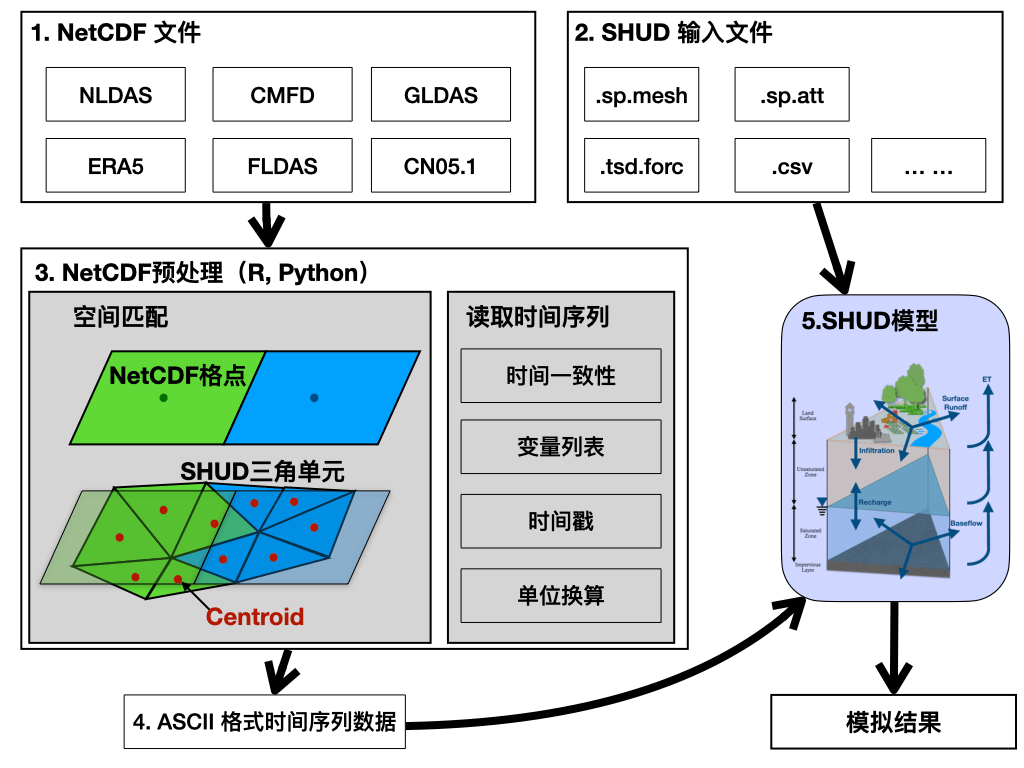
\includegraphics{_index.assets/NetCDF_module.003.png}
\caption{NetCDF\_module.003}
\end{figure}

本任务的目标是实现以下的方式:

\begin{figure}
\centering
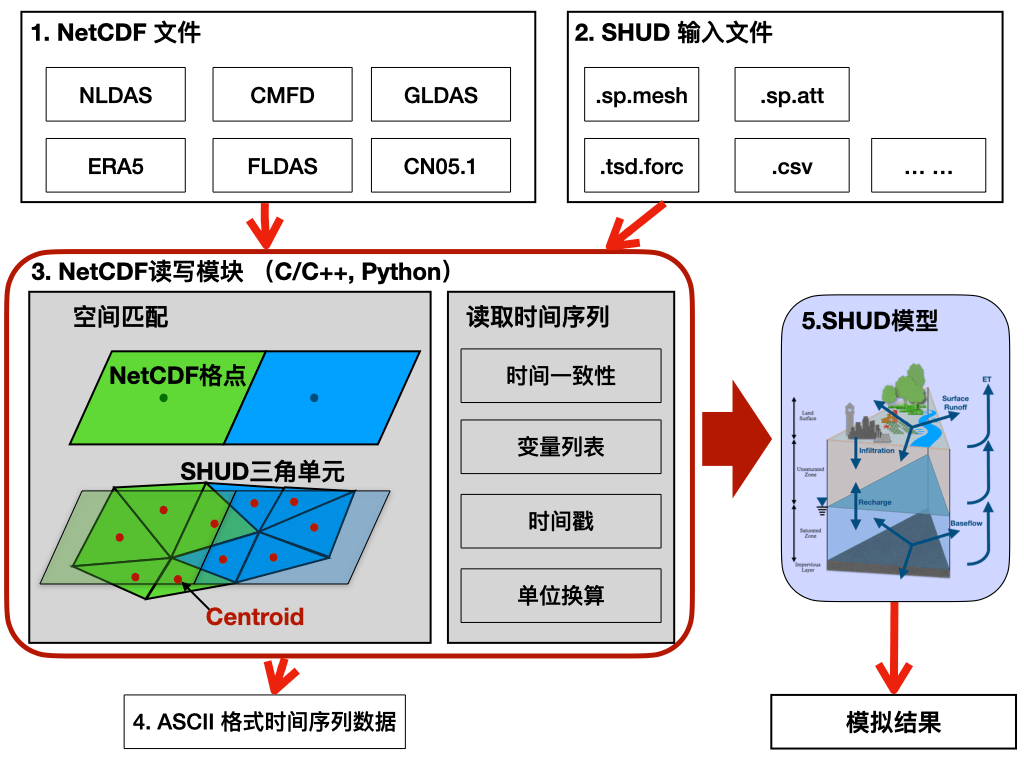
\includegraphics{_index.assets/NetCDF_module.002.png}
\caption{NetCDF\_module.002}
\end{figure}

技能要求:

\begin{enumerate}
\def\labelenumi{\arabic{enumi}.}
\tightlist
\item
  懂C/C++
\item
  能快速了解NetCDF数据结构。
\item
  了解GIS和空间数据。
\end{enumerate}

\hypertarget{d2.-ux751fux4ea7ux5168ux56fdux6c34ux6587ux6a21ux62dfux7cfbux7edfux7684ux8f93ux5165ux6570ux636e}{%
\subsubsection{\texorpdfstring{\textbf{D2. 生产全国水文模拟系统的输入数据}}{D2. 生产全国水文模拟系统的输入数据}}\label{d2.-ux751fux4ea7ux5168ux56fdux6c34ux6587ux6a21ux62dfux7cfbux7edfux7684ux8f93ux5165ux6570ux636e}}

我们已开发了全国水文模拟系统(\url{https://nwm.ac.cn}),但是这个系统中数据需要改进以提高计算效率和计算一致性。这一工作的路径非常清晰,但需要较多耐心去完成。

路径:

\begin{enumerate}
\def\labelenumi{\arabic{enumi}.}
\tightlist
\item
  系统性检查Shapefile河道数据。
\item
  对河道数据进行适度简化。
\item
  以全国流域片区对数据进行分解。
\item
  建立流域片区的SHUD模型输入文件。
\end{enumerate}

技能要求:

\begin{enumerate}
\def\labelenumi{\arabic{enumi}.}
\tightlist
\item
  懂GIS软件。
\item
  会空间数据分析。
\end{enumerate}

*\textbf{注:推荐有GIS经验的同学申请。}

\hypertarget{d2.-ux5168ux7403ux6c34ux6587ux4e91ux8ba1ux7b97ux5e73ux53f0ux4e2dux591aux6a21ux578bux96c6ux6210ux4efbux52a1}{%
\subsubsection{\texorpdfstring{\textbf{D2. 全球水文云计算平台中多模型集成任务}}{D2. 全球水文云计算平台中多模型集成任务}}\label{d2.-ux5168ux7403ux6c34ux6587ux4e91ux8ba1ux7b97ux5e73ux53f0ux4e2dux591aux6a21ux578bux96c6ux6210ux4efbux52a1}}

GHDC(\url{https://ghdc.ac.cn})网站可以为用户提供自动化的全球水文建模数据获取和水文建模任务,但是现在这个平台仅支持SHUD模型的自动化建模。因此本任务需要在当前网站数据流程框架下,开发其他模型支持模块,例如SWAT, TOPMODEL, 等等。

技能要求:

\begin{enumerate}
\def\labelenumi{\arabic{enumi}.}
\tightlist
\item
  精通Python, R之一。
\item
  懂水文建模,至少初步经验。
\end{enumerate}

\hypertarget{d3.-ux5168ux7403ux6c34ux6587ux4e91ux8ba1ux7b97ux5e73ux53f0ux4e2dapiux6d4bux8bd5ux548cux6539ux8fdbux4efbux52a1}{%
\subsubsection{\texorpdfstring{\textbf{D3. 全球水文云计算平台中API测试和改进任务}}{D3. 全球水文云计算平台中API测试和改进任务}}\label{d3.-ux5168ux7403ux6c34ux6587ux4e91ux8ba1ux7b97ux5e73ux53f0ux4e2dapiux6d4bux8bd5ux548cux6539ux8fdbux4efbux52a1}}

GHDC(\url{https://ghdc.ac.cn})网站可以为用户提供自动化的全球水文建模数据获取和水文建模任务。

GHDC服务支持网页和API方式提交数据,但是API模块仍然需要诸多的测试和改进。

技能要求:

\begin{enumerate}
\def\labelenumi{\arabic{enumi}.}
\tightlist
\item
  精通Python。
\item
  会用R。
\item
  会前台网页服务。
\end{enumerate}

*注:此任务有专业老师指导完成。

\hypertarget{d4.-ux5728ux8d85ux7b97ux4e0aux5b9eux73b0cma-esux591aux8282ux70b9ux5e76ux884cux7b97ux6cd5}{%
\subsubsection{\texorpdfstring{\textbf{D4. 在超算上实现CMA-ES多节点并行算法。}}{D4. 在超算上实现CMA-ES多节点并行算法。}}\label{d4.-ux5728ux8d85ux7b97ux4e0aux5b9eux73b0cma-esux591aux8282ux70b9ux5e76ux884cux7b97ux6cd5}}

当前我们在R上使用doParall和doMC将计算任务提交至超算允许,但是这种方式仅限单节点多线程并行计算。原因是R上doMC并行算法限制------即使申请了多节点计算资源,也无法调用多个节点,导致''一节点受难,多节点围观``的现象。

因此,我们需要一个新的脚本或者程序,将并行计算任务均匀分配到不同的计算节点上去。可以使用R或者Python实现。

技能要求:

\begin{enumerate}
\def\labelenumi{\arabic{enumi}.}
\tightlist
\item
  精通并行计算,知道多节点并行和单节点并行的区别。
\item
  精通R或者Python之一。
\end{enumerate}

\hypertarget{d5.-ux6d4bux8bd5ux548cux6539ux8fdbshudux6a21ux578bux7684openmpux5e76ux884cux7b97ux6cd5}{%
\subsubsection{\texorpdfstring{\textbf{D5. 测试和改进SHUD模型的OpenMP并行算法}}{D5. 测试和改进SHUD模型的OpenMP并行算法}}\label{d5.-ux6d4bux8bd5ux548cux6539ux8fdbshudux6a21ux578bux7684openmpux5e76ux884cux7b97ux6cd5}}

当前SHUD模型已经支持OpenMP并行算法,编译结果为shud-omp,但是其计算结果尚未经过验证。因此需要先将单线程的shud和多线程的shud-omp结果进行对比,确保多线程结果与单线程一致,进一步需要提升shud-omp的效率,寻找最优方案。

技能要求:

\begin{enumerate}
\def\labelenumi{\arabic{enumi}.}
\tightlist
\item
  精通并行计算。
\item
  精通C/C++。
\end{enumerate}

\hypertarget{ux5b66ux4e60ux8d44ux6e90}{%
\chapter{学习资源}\label{ux5b66ux4e60ux8d44ux6e90}}

下面是完成项目可用的资源:

\begin{itemize}
\tightlist
\item
  《SHUD研究组实验室手册》:网页版(\url{https://www.shud.xyz/book_lab/}), \href{https://www.shud.xyz/book_lab/_main.pdf}{PDF版本}, \href{https://www.shud.xyz/book_lab/_main.pdf}{ePub电子书版}.
\item
  R教程:\url{https://www.shud.xyz/bookr/}。大多数任务都要求申请者会使用R。通过本教程,你可以基本掌握R的使用,满足本组的R技能要求。
\item
  SHUD模型介绍:\url{https://www.shud.xyz/Book_CN/}
\item
  SHUD模型图库:\url{https://shudapp.netlify.app}
\item
  SHUD模型源代码:\url{https://github.com/SHUD-System/SHUD}
\item
  全球水文数据云(GHDC):网站(\url{https://ghdc.ac.cn/}),说明(\url{https://www.shud.xyz/ghdc_cn/}),\href{https://www.bilibili.com/video/BV1Km4y147Wz/?vd_source=50ff6ac37242c790173c755375aa0e4a}{Bilibili视频}。视频也可在Bilibili搜索``全球水文数据云平台(GHDC)''。
\item
  全国水文模拟系统(NWM):网站(\url{https://nwm.ac.cn})。
\end{itemize}

其他未尽事宜,可以直接联系PI舒乐乐:\href{mailto:shulele@lzb.ac.cn}{\nolinkurl{shulele@lzb.ac.cn}}。

  \bibliography{book.bib}

\end{document}
